\documentclass[]{memoir}
\title{Problem Set 3}
\author{Brian Fox}
\date{}
\usepackage{enumitem}
\usepackage{geometry}
\geometry{margin=35mm}
\usepackage{graphicx}
\usepackage{multicol}
\begin{document}
\maketitle

\begin{enumerate}
\item \textit{24.1-1} Run the Bellman-Ford algorithm on the directed graph of Figure 24.4, using vertex $z$ as the source. In each pass, relax edges in the same order as in the figure, and show the $d$ and $\pi$ values after each pass. Now, change the weight of edge $(z,x)$ to 4 and run the algorithm again, using $s$ as the source.
\paragraph{} fig 24.4:
\begin{figure}[h]
	\centering
	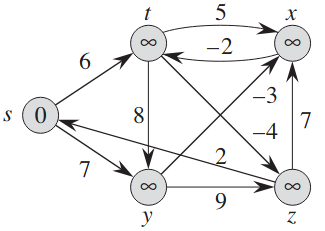
\includegraphics[scale=.7]{fig24-4}
\end{figure}

source z:\\
Initial
\begin{table}[h]
\begin{tabular}{l|l|l|l|l|l}
      & s        & t        & x        & y        & z   \\
$\pi$ & NIL      & NIL      & NIL      & NIL      & NIL \\
$d$   & $\infty$ & $\infty$ & $\infty$ & $\infty$ & 0  
\end{tabular}
\end{table}

first run 
\begin{table}[h!]
\begin{tabular}{l|l|l|l|l|l}
      & s   & t   & x   & y   & z   \\
$\pi$ & $z$ & $s$ & $z$ & $s$ & NIL \\
$d$   & 2   & 8   & 7   & 9   & 0  
\end{tabular}
\end{table}

second run
\begin{table}[h!]
\begin{tabular}{l|l|l|l|l|l}
      & s   & t   & x   & y   & z   \\
$\pi$ & $z$ & $x$ & $y$ & $s$ & NIL \\
$d$   & 2   & 5   & 6   & 9   & 0  
\end{tabular}
\end{table}
\pagebreak
\\
third run
\begin{table}[h!]
\begin{tabular}{l|l|l|l|l|l}
      & s   & t   & x   & y   & z   \\
$\pi$ & $z$ & $x$ & $y$ & $s$ & NIL \\
$d$   & 2   & 4   & 6   & 9   & 0  
\end{tabular}
\end{table}

fourth run
\begin{table}[h!]
\begin{tabular}{l|l|l|l|l|l}
      & s   & t   & x   & y   & z   \\
$\pi$ & $z$ & $x$ & $y$ & $s$ & NIL \\
$d$   & 2   & 4   & 6   & 9   & 0  
\end{tabular}
\end{table}

source $s$, $w(z,x)=4$:
Initial
\begin{table}[h]
\begin{tabular}{l|l|l|l|l|l}
      & s        & t        & x        & y        & z   \\
$\pi$ & NIL      & NIL      & NIL      & NIL      & NIL \\
$d$   & 0        & $\infty$ & $\infty$ & $\infty$ & $\infty$
\end{tabular}
\end{table}

first run
\begin{table}[h]
\begin{tabular}{l|l|l|l|l|l}
      & s        & t   & x        & y   & z   \\
$\pi$ & NIL      & $s$ & NIL      & $s$ & NIL \\
$d$   & 0        & 6   & $\infty$ & 7   & $\infty$
\end{tabular}
\end{table}
\pagebreak
\\
second run
\begin{table}[h]
\begin{tabular}{l|l|l|l|l|l}
      & s        & t   & x   & y   & z   \\
$\pi$ & NIL      & $s$ & $y$ & $s$ & $t$ \\
$d$   & 0        & 6   & 4   & 7   & 2
\end{tabular}
\end{table}

third run
\begin{table}[h]
\begin{tabular}{l|l|l|l|l|l}
      & s        & t   & x   & y   & z   \\
$\pi$ & NIL      & $x$ & $y$ & $s$ & $t$ \\
$d$   & 0        & 2   & 4   & 7   & 2
\end{tabular}
\end{table}

fourth run
\begin{table}[h]
\begin{tabular}{l|l|l|l|l|l}
      & s        & t   & x   & y   & z   \\
$\pi$ & NIL      & $x$ & $z$ & $s$ & $t$ \\
$d$   & 0        & 2   & 2   & 7   & -2
\end{tabular}
\end{table}

\item \textit{24.2-1} Run DAG-SHORTEST-PATHS on the directed graph of Figure 24.5, using vertex $r$ as the source.
\paragraph{} fig 24.5:
\begin{figure}[h]
	\centering
	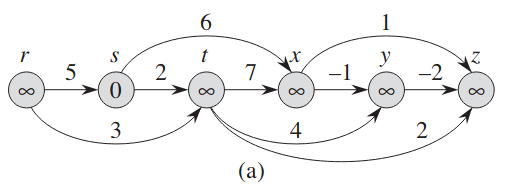
\includegraphics[scale=.7]{fig24-5}
\end{figure}
\pagebreak\\
Initial
\begin{table}[h]
\begin{tabular}{l|l|l|l|l|l|l}
      & r        & s        & t        & x        & y        & z   \\
$\pi$ & NIL      & NIL      & NIL      & NIL      & NIL      & NIL \\
$d$   & $\infty$ & 0        & $\infty$ & $\infty$ & $\infty$ & $\infty$
\end{tabular}
\end{table}

relax $r$'s adjacency list
\begin{table}[h]
\begin{tabular}{l|l|l|l|l|l|l}
      & r        & s        & t        & x        & y        & z   \\
$\pi$ & NIL      & NIL      & NIL      & NIL      & NIL      & NIL \\
$d$   & $\infty$ & 0        & $\infty$ & $\infty$ & $\infty$ & $\infty$
\end{tabular}
\end{table}

relax $s$'s adjacency list
\begin{table}[h]
\begin{tabular}{l|l|l|l|l|l|l}
      & r        & s        & t   & x   & y        & z   \\
$\pi$ & NIL      & NIL      & $s$ & $s$ & NIL      & NIL \\
$d$   & $\infty$ & 0        & 2   & 6   & $\infty$ & $\infty$
\end{tabular}
\end{table}

relax $t$'s adjacency list
\begin{table}[h]
\begin{tabular}{l|l|l|l|l|l|l}
      & r        & s        & t   & x   & y   & z   \\
$\pi$ & NIL      & NIL      & $s$ & $s$ & $t$ & $t$ \\
$d$   & $\infty$ & 0        & 2   & 6   & 6   & 4
\end{tabular}
\end{table}
\pagebreak\\
relax $x$'s adjacency list
\begin{table}[h]
\begin{tabular}{l|l|l|l|l|l|l}
      & r        & s        & t   & x   & y   & z   \\
$\pi$ & NIL      & NIL      & $s$ & $s$ & $x$ & $t$ \\
$d$   & $\infty$ & 0        & 2   & 6   & 5   & 4
\end{tabular}
\end{table}

relax $y$'s adjacency list
\begin{table}[h]
\begin{tabular}{l|l|l|l|l|l|l}
      & r        & s        & t   & x   & y   & z   \\
$\pi$ & NIL      & NIL      & $s$ & $s$ & $x$ & $y$ \\
$d$   & $\infty$ & 0        & 2   & 6   & 5   & 3
\end{tabular}
\end{table}

\item \textit{24.3-1} Run Dijkstra’s algorithm on the directed graph of Figure 24.2, first using vertex $s$ as the source and then using vertex $z$ the source. In the style of Figure 24.6, show the $d$ and $\pi$ values and the vertices in set $S$ after each iteration of the \textbf{while} loop.
\paragraph{} fig 24.2:
\begin{figure}[h]
	\centering
	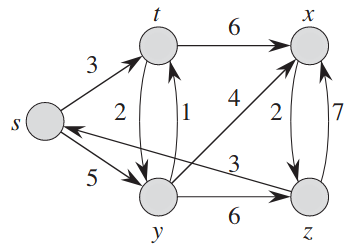
\includegraphics[scale=.7]{fig24-2}
\end{figure}
source s:
\begin{figure}[h]
	\centering
	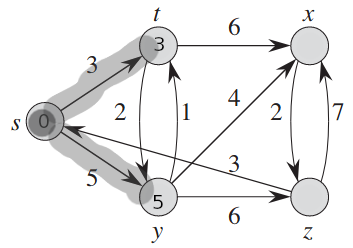
\includegraphics[scale=.7]{s1}
\end{figure}
\begin{figure}[h]
	\centering
	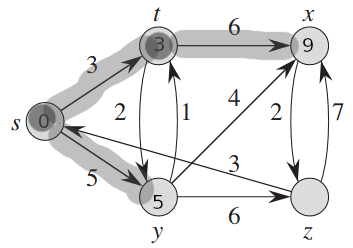
\includegraphics[scale=.7]{s2}
\end{figure}
\begin{figure}[h]
	\centering
	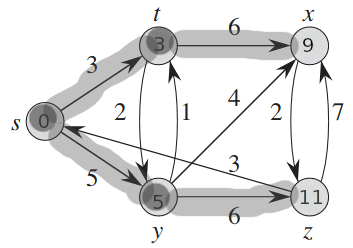
\includegraphics[scale=.7]{s3}
\end{figure}
\begin{figure}[h]
	\centering
	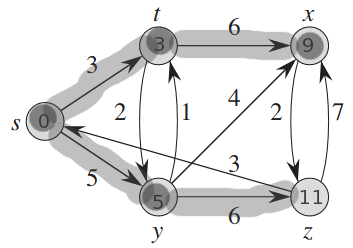
\includegraphics[scale=.7]{s4}
\end{figure}
\begin{figure}[h]
	\centering
	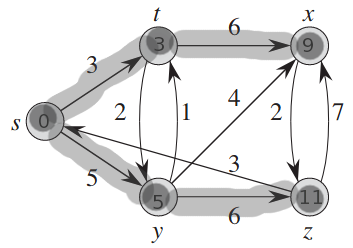
\includegraphics[scale=.7]{s5}
\end{figure}
\pagebreak\\
source z:
\begin{figure}[h]
	\centering
	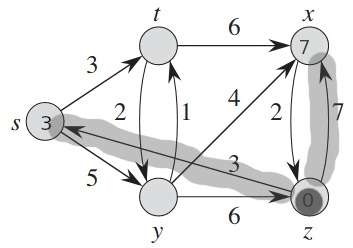
\includegraphics[scale=.7]{z1}
\end{figure}
\begin{figure}[h]
	\centering
	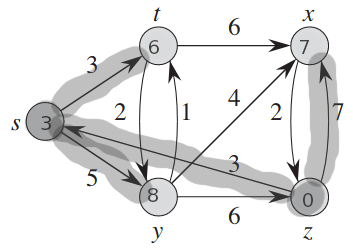
\includegraphics[scale=.7]{z2}
\end{figure}
\begin{figure}[h]
	\centering
	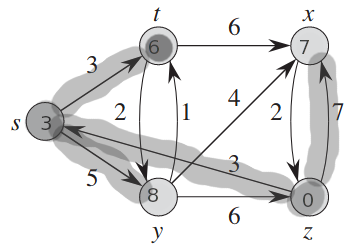
\includegraphics[scale=.7]{z3}
\end{figure}
\begin{figure}[h]
	\centering
	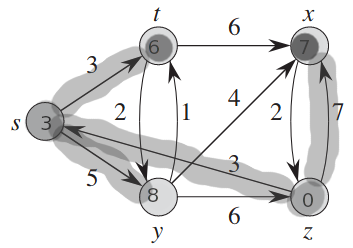
\includegraphics[scale=.7]{z4}
\end{figure}
\begin{figure}[h]
	\centering
	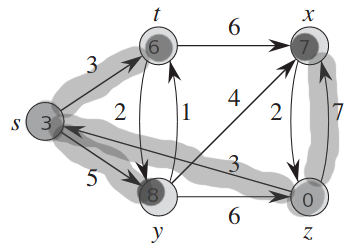
\includegraphics[scale=.7]{z5}
\end{figure}

\end{enumerate}
\end{document}

